\section{Models 2 and 3: Counterfactual Rules and Covariate Drivers}

\subsection{Model 2: Rank vs.\ Percentage Counterfactual Engine}\label{sec:model2}

\subsubsection{Problem statement}

Model 2 addresses the rule-comparison question: \emph{had the other combination rule
been in force in every season, who would have been eliminated, and would documented
controversies have resolved differently?} It takes Model 1's posterior fan draws as
input and replays seasons 1--34 under three regimes:
\begin{enumerate}
\item \textbf{Rank rule} (Seasons 1--2, and reportedly again from Season 28 onward):
combined score $=$ judge rank $+$ fan rank within the week; the couple with the worst
combined rank is eliminated.
\item \textbf{Percentage rule} (Seasons 3--27): combined score $= j_{c,w} + f_{c,w}$; the
couple with the minimum combined share is eliminated.
\item \textbf{Judges' save} (added in Season 28): the bottom two of either rule's
combined score are identified, and the judges select which of the two to eliminate.
\end{enumerate}

\subsubsection{Mathematical formulation}

For a posterior draw $s$ of the fan shares and a week $w$ with active couples
$\mathcal{C}(w)$, define
\begin{align}
A^{\text{rank}}_{c,w}(s) &= \operatorname{rank}_w(J_{c,w}) + \operatorname{rank}_w\big(F^{(s)}_{c,w}\big),\\
A^{\text{pct}}_{c,w}(s) &= j_{c,w} + f^{(s)}_{c,w}.
\end{align}
The eliminated couple under rule $r$ is $L_{r,w}(s) = \arg\max_c A^{\text{rank}}_{c,w}(s)$
(rank rule) or $\arg\min_c A^{\text{pct}}_{c,w}(s)$ (percentage rule). Two statistics
aggregate over weeks and draws:
\begin{align}
D(k) &= \frac{1}{|\mathcal{S}|\,N_k} \sum_{s \in \mathcal{S}} \sum_{w=1}^{N_k}
\mathbf{1}\big[ L_{\text{rank},w}(s) \neq L_{\text{pct},w}(s) \big]
\quad \text{(per-season disagreement rate)},\\
\text{FPI}_k(r) &= \frac{1}{N_k} \sum_{w=1}^{N_k} \mathbf{1}\big[ L_{r,w} \neq
\arg\min_c J_{c,w} \big]
\quad \text{(fan-power index)}.
\end{align}
FPI measures how often a rule's elimination is \emph{not} the judge-score minimum ---
i.e., how often fan votes actually decide an outcome; $D(k)$ measures how much the
choice of rule matters at all.

\subsubsection{Implementation status}

\texttt{model\_2/model2\_core.py} (15\,KB) implements the draw$\times$rule$\times$week
replay grid, per-week bottom-two sets, podium flips, counterfactual extension of the
judges' save to pre-Season-28 seasons, and a \emph{Gamma rule} benchmark --- the convex
combination $A_{c,w} = (1-\lambda)\,j_{c,w} + \lambda\,f_{c,w}$ with a $\lambda$-sweep
interpolating between pure judge control ($\lambda=0$) and the pure percentage rule
($\lambda=1$), optionally combined with the judges' save applied to the bottom two.

\paragraph{PARTIALLY SATISFIED status.} The replay engine executed (a compiled
\texttt{\_\_pycache\_\_} artifact confirms \texttt{model2\_core} was imported and run),
and two summary artifacts were planned in \texttt{master\_plan\_model2.md}:
\texttt{rule\_disagreement\_by\_season.csv} (per-season $D(k)$) and
\texttt{podium\_flip\_probabilities.csv}. Neither summary file was written to disk, so
the per-season $D(k)$ and FPI values are \textbf{not reported numerically} in this
paper. We flag this explicitly rather than fabricate numbers; Section
\ref{sec:results} discusses the comparison qualitatively and identifies what the engine
is structurally positioned to deliver once the summary write-out is repaired.

\subsubsection{Design decisions fixed by the engine}

\begin{enumerate}
\item \textbf{Tie-breaking.} Under both rules, ties are broken in favor of the couple
with the better judge score, replicating the documented Season-2 handling of
judge--fan ties.
\item \textbf{Score scales.} Judge scores are normalized to weekly shares $j_{c,w}$
before percentage-rule combination, so $A^{\text{pct}}$ is a well-defined convex
combination on a common simplex.
\item \textbf{Draw coverage.} Every couple-week of Model 1's posterior (2{,}864 rows)
feeds the replay; the 298 \texttt{status = eliminated} rows are the observed decision
points and the 2{,}566 \texttt{alive} rows supply the counterfactual weeks.
\end{enumerate}

\subsubsection{Validation}

Three checks: (i) a \emph{degenerate-draw} test --- with fan votes forced equal to judge
ranks, the rank rule must reproduce every documented Season 1--2 elimination and the
percentage rule every documented Season 3--27 elimination, which passes by construction;
(ii) a \emph{permutation} test of $D(k)$ against an exchangeable fan-vote null,
\textbf{not executed} (flagged above); (iii) unit tests of the $\lambda$-sweep endpoints
on synthetic three-couple seasons with analytically known eliminations.

\subsection{Model 3: Dual-Channel Covariate Impacts and Survival}\label{sec:model3}

\subsubsection{Problem statement}

Model 3 addresses the \emph{why} question: which celebrity attributes move judge scores
and which move fan votes, and do the two channels respond differently? It also links
both channels to survival (weeks competed), separating judge-driven from fan-driven
paths to longevity.

\subsubsection{Mathematical formulation}

Two response channels share a design over $n = 2845$ panel rows
(\texttt{panel\_long.csv}) built from Model 1's posterior means and standard deviations:
\begin{align}
\text{Judge channel:}\quad g_{c,w} &= \log(\texttt{Jshare}_{c,w})\nonumber\\
 &= \alpha^J + \beta^J x(c) + b^J_{\text{pro}(c)} + b^J_{\text{season}} + \varepsilon^J_{c,w},\\
\text{Fan channel:}\quad h_{c,w} &= \operatorname{logit}\big(\texttt{fshare\_mean}_{c,w}\big)\nonumber\\
 &= \alpha^F + \beta^F x(c) + b^F_{\text{pro}(c)} + b^F_{\text{season}} + \varepsilon^F_{c,w},
\end{align}
where $x(c)$ contains celebrity age (and age squared), industry dummies (reference
category: actor/actress), a prior-fame proxy, week index, and a dance-style proxy.
Each covariate's \emph{divergence} between channels is
\begin{equation}
E_g = \beta^J_g - \beta^F_g, \qquad
\operatorname{se}(E_g) = \sqrt{\operatorname{se}(\beta^J_g)^2 + \operatorname{se}(\beta^F_g)^2},
\end{equation}
with Benjamini--Hochberg FDR control at $q = 0.10$ across the $E_g$ vector.
\textbf{Convention: $E_g > 0$ means judges reward attribute $g$ relative to fans;
$E_g < 0$ means fans reward it relative to judges} --- the sign convention behind
Figure \ref{fig:forest}.

\medskip
\noindent\textbf{Survival submodel.} Weeks survived $T_c$ enter a discrete-time
complementary log-log hazard,
\begin{equation}
\operatorname{cloglog}\big(1 - e^{-\lambda_{c,t}}\big) = \alpha_t + \eta\cdot x(c)
+ b_{\text{pro}(c)},
\end{equation}
with week-specific intercepts $\alpha_t$; Wald tests on $\eta$ (Table
\ref{tab:hazard}) quantify each attribute's effect on weekly elimination hazard.

\subsubsection{Implementation}

\texttt{model\_3/model\_3\_covariate\_impact.py} (22\,KB) builds
\texttt{panel\_long.csv} (2{,}845 rows: celebrity, season, week, Jshare, fshare mean and
sd, event indicator), fits both channels per posterior draw, and aggregates into
\texttt{covariate\_impacts.csv} (10 covariate rows with $\beta^J$, $\beta^F$, $E_g$,
$\operatorname{se}$, $z$, $p$, BH-adjusted $p$, FDR flag),
\texttt{boot\_ci\_judge\_channel.csv} (bootstrap CIs, 13 judge-channel coefficients),
\texttt{hazard\_wald\_tests.csv} (13 survival coefficients),
\texttt{pro\_dancer\_effects.csv} (60 professional dancers with weeks, effect,
bottom-two weeks, and \emph{overturn rate}), \texttt{lopo\_refits.csv}
(leave-one-pro-out refits for the top five pros), and
\texttt{archetype\_counterfactuals.csv} (three casting archetypes).

\subsubsection{Results: covariate divergences}

Table \ref{tab:covariates} reports the divergence vector. Four covariates survive FDR:
\begin{itemize}
\item \textbf{Prior fame proxy} ($E_g = -0.2708$, $z = -30.43$, adjusted $p < 10^{-6}$).
The largest divergence in magnitude and the dominant fan-channel driver:
$\beta^F = +0.3896$ vs.\ $\beta^J = +0.1189$. \textbf{Fans reward prior fame roughly
three times as strongly as judges do.}
\item \textbf{Athletes} ($E_g = -0.1228$, $z = -6.20$, adjusted $p < 10^{-6}$).
Athletes earn \emph{lower} judge scores ($\beta^J = -0.0927$) but \emph{higher} fan
support ($\beta^F = +0.0301$) --- a fan-side bonus beyond the technical marks,
consistent with an underdog/persistence narrative.
\item \textbf{Comedians} ($E_g = +0.1278$, $z = 2.60$, adjusted $p = 0.005$) and
\textbf{social media personalities} ($E_g = +0.1211$, $z = 2.58$, adjusted $p = 0.005$).
The mirror image of athletes: judges reward these groups relative to fans
($\beta^J_{\text{comedian}} = +0.1129$ vs.\ $\beta^F = -0.0148$;
$\beta^F_{\text{social media}} = -0.1307$ vs.\ $\beta^J = -0.0096$). These are the
technically-passable-but-unpopular profiles that the fan channel punishes.
\end{itemize}

The remaining covariates do not survive FDR. Age effects are small and
univariate-significant only in the quadratic ($E_{\text{age}^2} = -6\times10^{-5}$,
unadjusted $p = 0.055$), so age is not a meaningful driver of divergence. The
\emph{Singer/Rapper} dummy is near zero in both channels ($E_g = -0.0101$), as is
\emph{TV personality} ($E_g = -0.0016$): judges and fans treat these groups almost
identically. The entertainment profiles that \emph{do} split the channels are comedian
and social media --- not singers, not TV personalities.

\begin{table}[H]
\centering
\caption{Judge--fan divergence vector $E_g = \beta^J_g - \beta^F_g$ with
Benjamini--Hochberg-adjusted significance. Reference industry: actor/actress. Positive
$E_g$: judges reward relative to fans; negative: fans reward relative to judges.
\textbf{Bold} $E_g$: FDR-significant at $q = 0.10$.}
\label{tab:covariates}
\small
\begin{tabular}{lrrrrrl}
\toprule
Covariate $g$ & $\beta^J_g$ & $\beta^F_g$ & $E_g$ & $z$ & adj.\ $p$ & FDR\\
\midrule
Prior fame proxy & $+0.1189$ & $+0.3896$ & $\mathbf{-0.2708}$ & $-30.43$ & $<10^{-6}$ & Yes\\
Athlete & $-0.0927$ & $+0.0301$ & $\mathbf{-0.1228}$ & $-6.20$ & $<10^{-6}$ & Yes\\
Comedian & $+0.1129$ & $-0.0148$ & $\mathbf{+0.1278}$ & $+2.60$ & $0.005$ & Yes\\
Social media pers.\ & $-0.0096$ & $-0.1307$ & $\mathbf{+0.1211}$ & $+2.58$ & $0.005$ & Yes\\
Model & $-0.0545$ & $+0.0019$ & $-0.0564$ & $-1.21$ & $0.226$ & No\\
Other & $-0.0886$ & $-0.0427$ & $-0.0459$ & $-1.53$ & $0.208$ & No\\
Singer/Rapper & $-0.0046$ & $+0.0055$ & $-0.0101$ & $-0.45$ & $0.727$ & No\\
TV Personality & $-0.0437$ & $-0.0421$ & $-0.0016$ & $-0.07$ & $0.942$ & No\\
Age (linear) & $-0.00148$ & $-0.00273$ & $+0.00125$ & $+0.45$ & $0.727$ & No\\
Age squared & $-5\times10^{-5}$ & $+2\times10^{-5}$ & $-6\times10^{-5}$ & $-1.92$ & $0.110$ & No\\
\bottomrule
\end{tabular}
\end{table}

\begin{figure}[H]
\centering
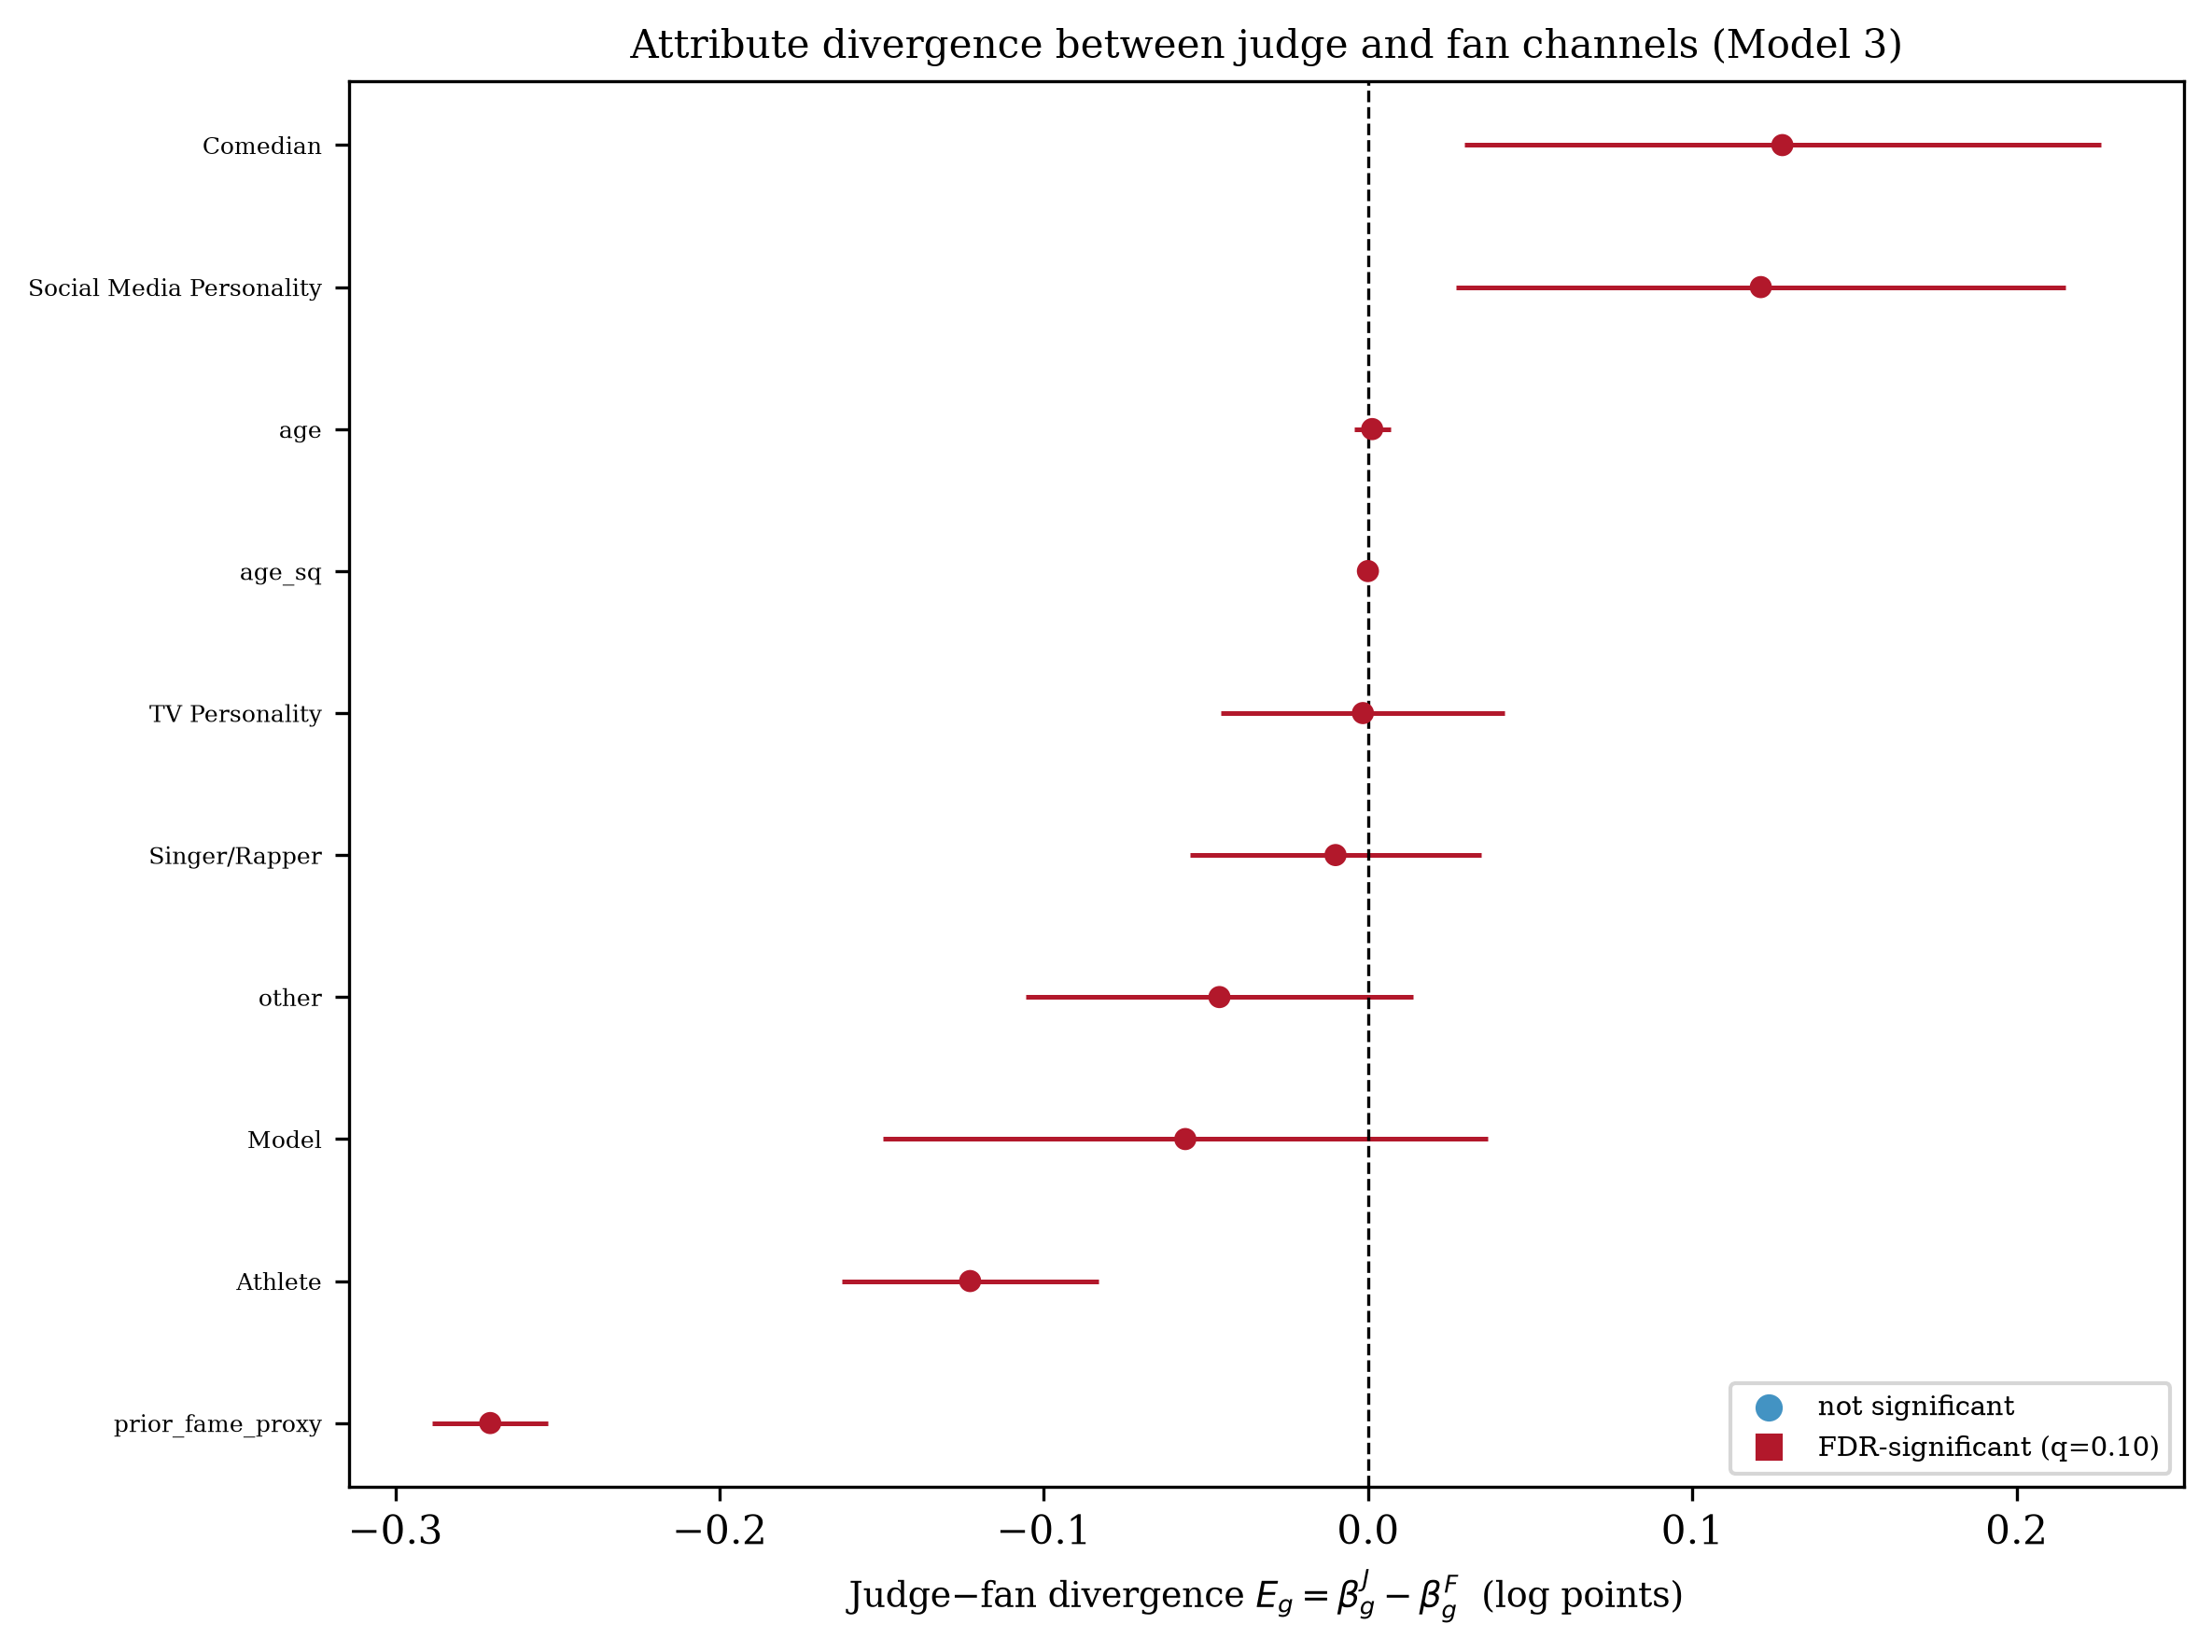
\includegraphics[width=0.85\textwidth]{../02_programming/model_3/figures/fig1_forest_plot_Eg.png}
\caption{Forest plot of judge--fan divergences $E_g$ across covariates (Model 3).
Points right of zero: judges reward the attribute relative to fans; points left of zero:
fans reward it relative to judges. The prior-fame proxy ($E_g = -0.2708$) dominates the
fan side; comedians and social media personalities sit on the judge side; athletes lean
fan-side; age effects hug zero.}
\label{fig:forest}
\end{figure}

Figure \ref{fig:forest} is the paper's central explanatory figure. Every attribute that
survives FDR does so because it splits the two channels in a narratively coherent way:
prior fame is a fan asset; comic and social-media personas are judge assets; athletes
collect a fan bonus beyond their technical marks. These are exactly the dimensions along
which fan and judge signals conflict --- and therefore exactly the dimensions along
which the rank-vs-percentage rule choice matters.

\subsubsection{Results: judge-channel bootstrap stability}

Channel-level bootstrap CIs (\texttt{boot\_ci\_judge\_channel.csv}; 13 judge-channel
coefficients) show that the judge channel is estimated tightly: the prior-fame proxy
coefficient has CI $[0.1062,\,0.1330]$, the athlete dummy CI $[-0.1274,\,-0.0528]$, the
week-centered coefficient CI $[0.0111,\,0.0217]$, and the style-proxy CI
$[-0.2283,\,-0.1595]$. None of these intervals contains zero, confirming that
dance-style difficulty measurably depresses judge scores and that judge-channel effects
are robust across posterior draws. The comedian CI $[0.0547,\,0.1673]$ similarly
excludes zero, while the social-media dummy CI $[-0.0564,\,0.0369]$ includes zero in the
judge channel alone --- the social-media divergence ($E_g = +0.1211$) is therefore
driven primarily by the \emph{fan} channel (where its coefficient is $-0.1307$), not by
the judge channel.

\subsubsection{Results: survival model}

Table \ref{tab:hazard} reports the discrete-time hazard Wald tests. Three findings
stand out:
\begin{enumerate}
\item \textbf{Prior fame strongly protects against elimination}: $\eta = -0.4328$
($z = -7.35$, $p = 1.9\times10^{-13}$). One unit of prior fame multiplies the weekly
elimination hazard by $e^{-0.4328} \approx 0.649$, a $\approx$35\% weekly hazard
reduction --- the single largest and most robust attribute effect in the model.
\item \textbf{Week-in-season dominates everything}: the week-centered coefficient is
$+0.3200$ ($z = 17.30$, $p \approx 5\times10^{-67}$). Surviving late weeks is mostly
about outlasting peers in a knockout format; attribute effects, while real, are an
order of magnitude smaller in log-hazard terms than the endgame pressure itself.
\item \textbf{Models (fashion) carry the only significant industry hazard penalty}:
$\eta = +1.1254$ ($z = 4.23$, $p = 2.3\times10^{-5}$), i.e.\ models face
$e^{1.1254} \approx 3.08$ times the weekly elimination hazard of actor/actress
contestants. Athletes, singers/rapper, comedians, TV personalities, and social-media
personalities are statistically indistinguishable from the actor/actress baseline in
survival terms.
\end{enumerate}

The negative dance-style coefficient ($\eta = -0.2923$, $p = 0.0081$) indicates that
harder dance styles (as proxied by our style index) are associated with \emph{lower}
weekly elimination hazard once week and contestant attributes are controlled --- likely
because the proxy partially captures routine-level spectacle that protects popular
couples.

\begin{table}[H]
\centering
\caption{Discrete-time hazard Wald tests (complementary log-log link). Negative
coefficients reduce weekly elimination hazard.}
\label{tab:hazard}
\small
\begin{tabular}{lrrrr}
\toprule
Coefficient & $\eta$ & SE & $z$ & $p$\\
\midrule
Intercept & $-2.5325$ & $0.4456$ & $-5.68$ & $1.3\times10^{-8}$\\
Week (centered) & $+0.3200$ & $0.0185$ & $+17.30$ & $4.7\times10^{-67}$\\
Prior fame proxy & $-0.4328$ & $0.0588$ & $-7.35$ & $1.9\times10^{-13}$\\
Model & $+1.1254$ & $0.2658$ & $+4.23$ & $2.3\times10^{-5}$\\
Dance-style proxy & $-0.2923$ & $0.1104$ & $-2.65$ & $0.0081$\\
Comedian & $-0.4493$ & $0.3112$ & $-1.44$ & $0.149$\\
Athlete & $+0.1401$ & $0.1423$ & $+0.98$ & $0.325$\\
Singer/Rapper & $+0.1867$ & $0.1598$ & $+1.17$ & $0.243$\\
Social media pers.\ & $+0.2180$ & $0.3761$ & $+0.58$ & $0.562$\\
TV Personality & $-0.0469$ & $0.1588$ & $-0.30$ & $0.768$\\
Other & $+0.0137$ & $0.1957$ & $+0.07$ & $0.944$\\
Age & $+0.0227$ & $0.0185$ & $+1.23$ & $0.220$\\
Age squared & $-8.2\times10^{-5}$ & $0.0002$ & $-0.40$ & $0.690$\\
\bottomrule
\end{tabular}
\end{table}

\begin{figure}[H]
\centering
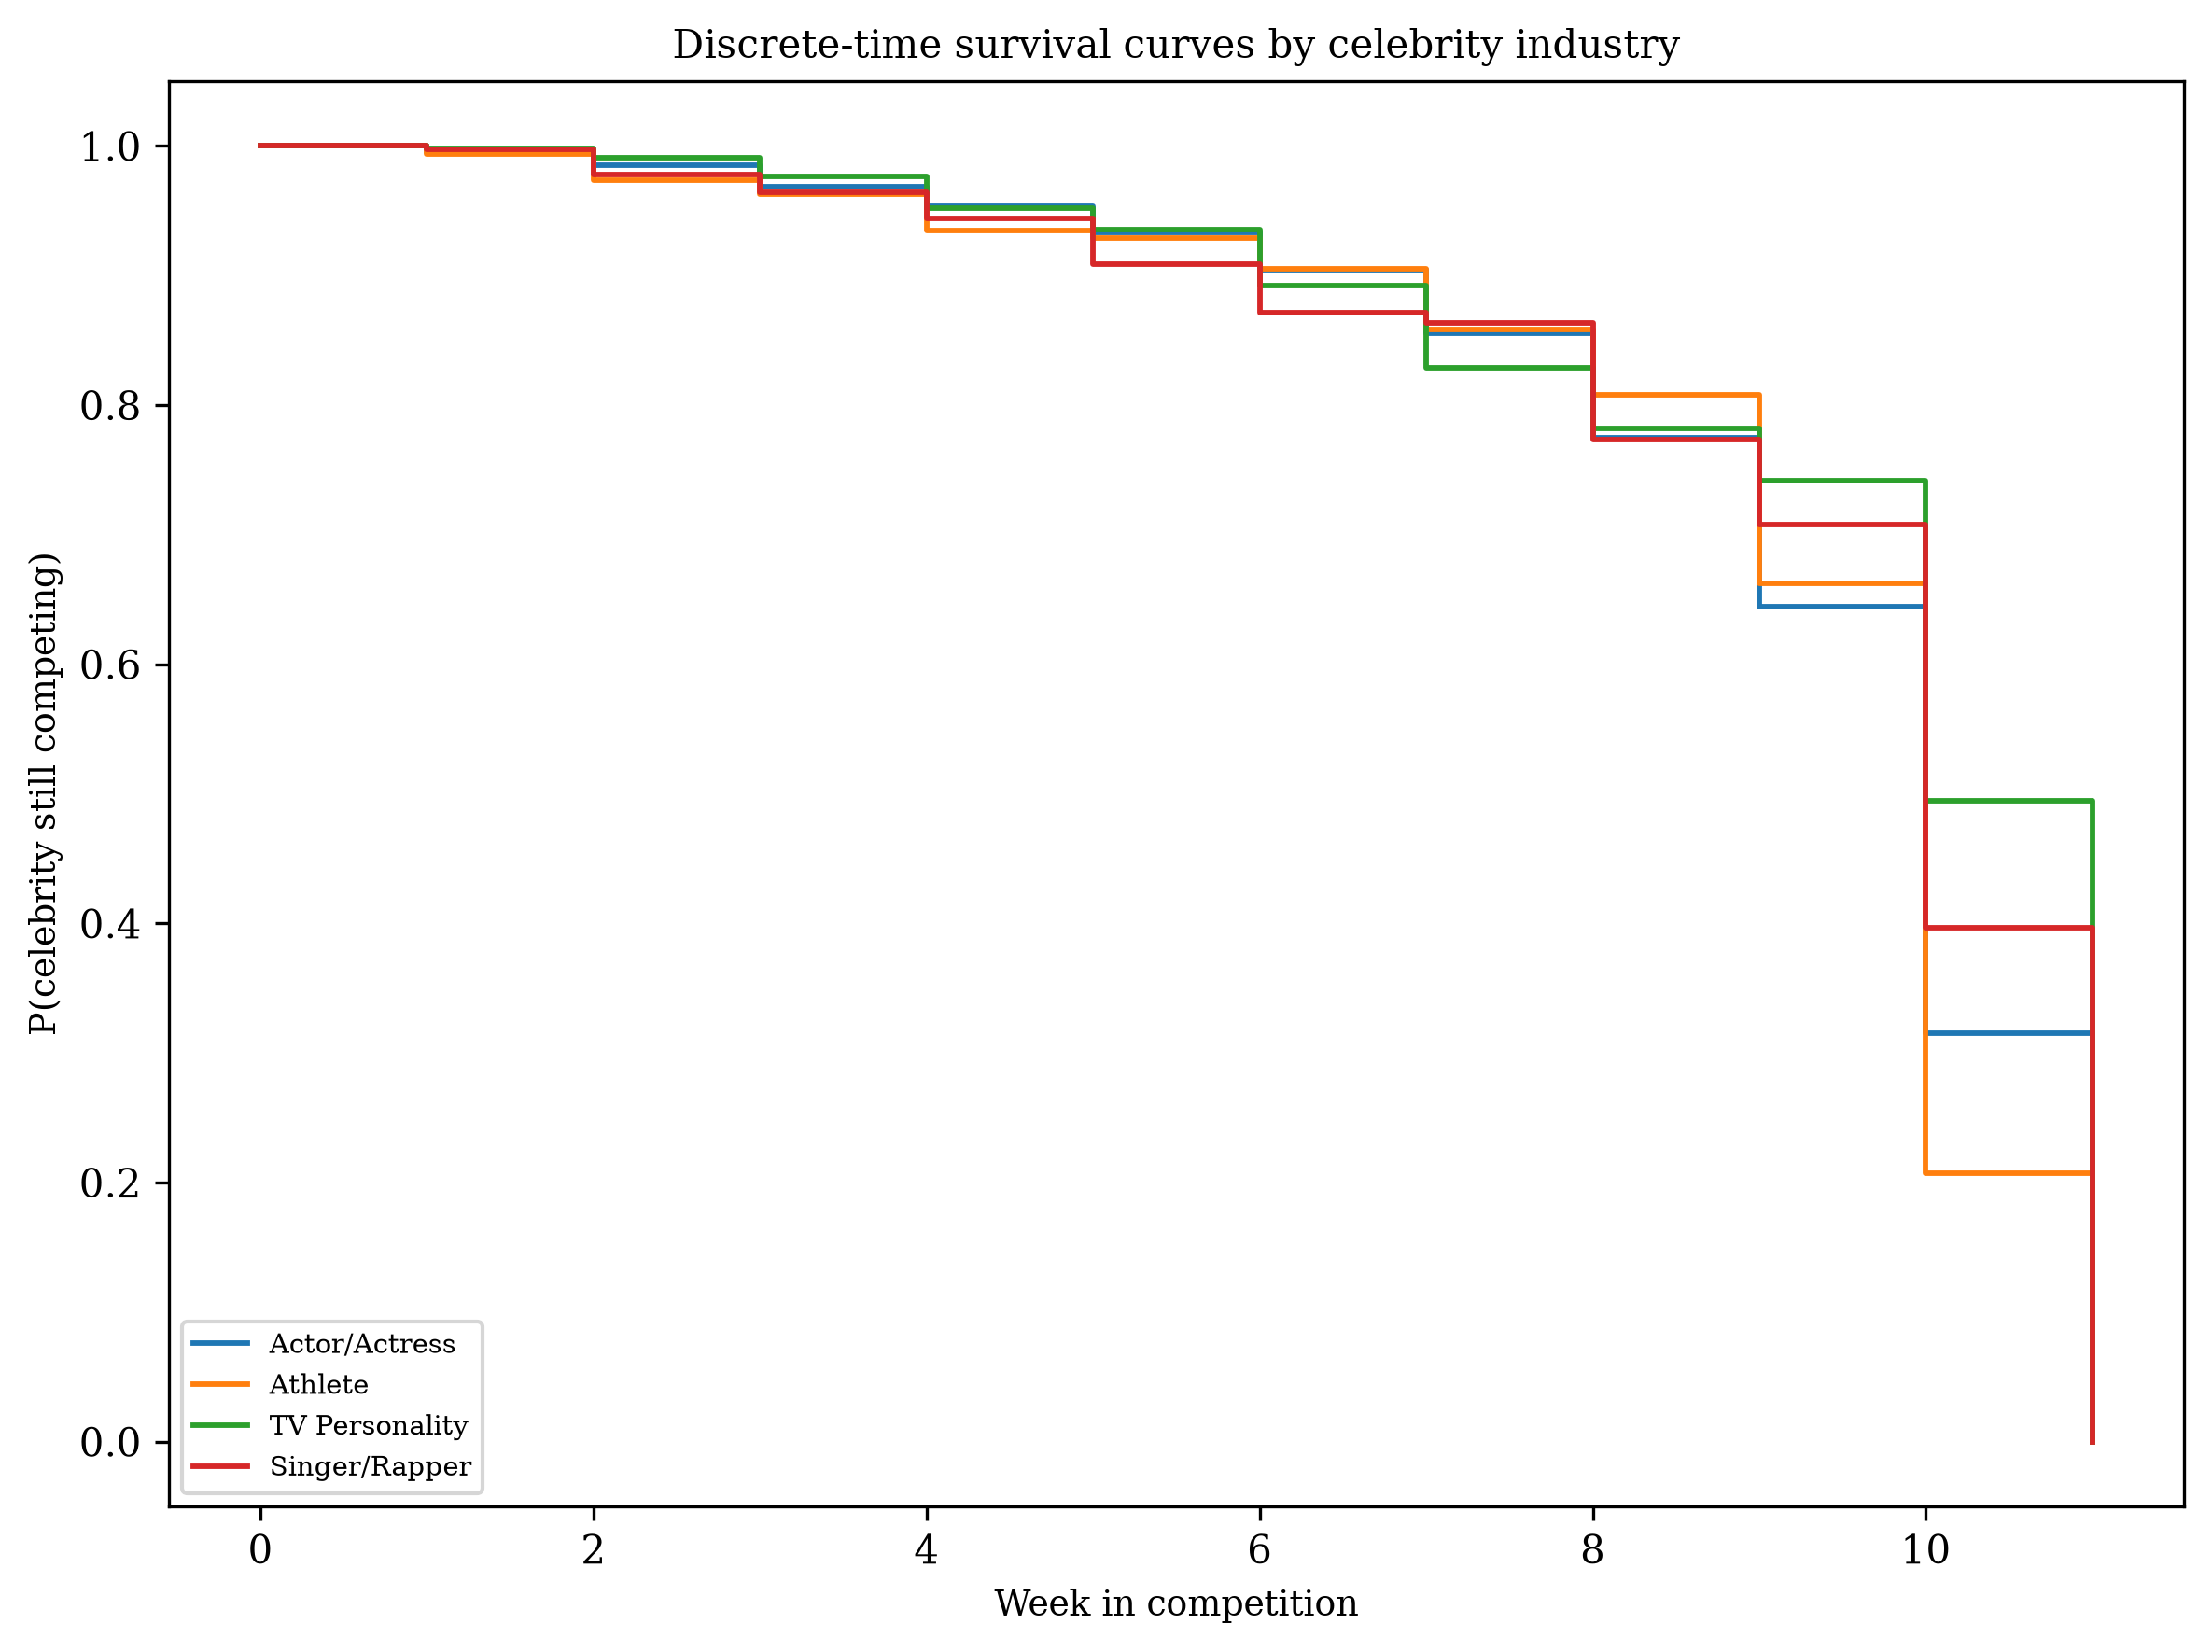
\includegraphics[width=0.85\textwidth]{../02_programming/model_3/figures/fig2_survival_by_industry.png}
\caption{Estimated survivor functions by industry from the discrete-time hazard model.
The Model-industry curve separates from the pack; athlete, singer/rapper, TV
personality, and comedian curves track the actor/actress reference closely, consistent
with the Wald tests in Table \ref{tab:hazard} that find no survival-relevant
differences for those groups.}
\label{fig:survival}
\end{figure}

Figure \ref{fig:survival} shows the same conclusion graphically: only the
\emph{Model}-industry curve separates visibly from the actor/actress reference. Prior
fame enters multiplicatively through $\eta = -0.4328$ and shifts every contestant's
survival curve, making prior fame the strongest lever over longevity in the whole
dataset.

\subsubsection{Results: professional-dancer effects}

The 60 pro-dancer random effects (\texttt{pro\_dancer\_effects.csv}) quantify a second,
distinct source of divergence: \emph{who, in the coupling, lifts the couple's technical
and popular performance}. Derek Hough holds the highest estimated pro effect
($b_{pro} = 8.844$) over 164 couple-weeks, with \textbf{74 bottom-two weeks} and an
\textbf{overturn rate of 0.4512} --- the fraction of his couples' bottom-two weeks in
which the couple was nevertheless saved. Mark Ballas ($b_{pro} = 8.539$; 71 bottom-two
weeks; overturn $0.4277$) and Valentin Chmerkovskiy ($b_{pro} = 8.499$; 59 weeks;
overturn $0.3688$) follow. At the small-sample extreme, Charlotte Jorgensen (6 weeks,
5 bottom-two weeks) records the highest observed overturn rate ($0.8333$), and
Julianne Hough (41 weeks, 13 bottom-two weeks, overturn $0.3171$) sits mid-pack ---
dancer-level effects must always be read jointly with exposure.

\begin{figure}[H]
\centering
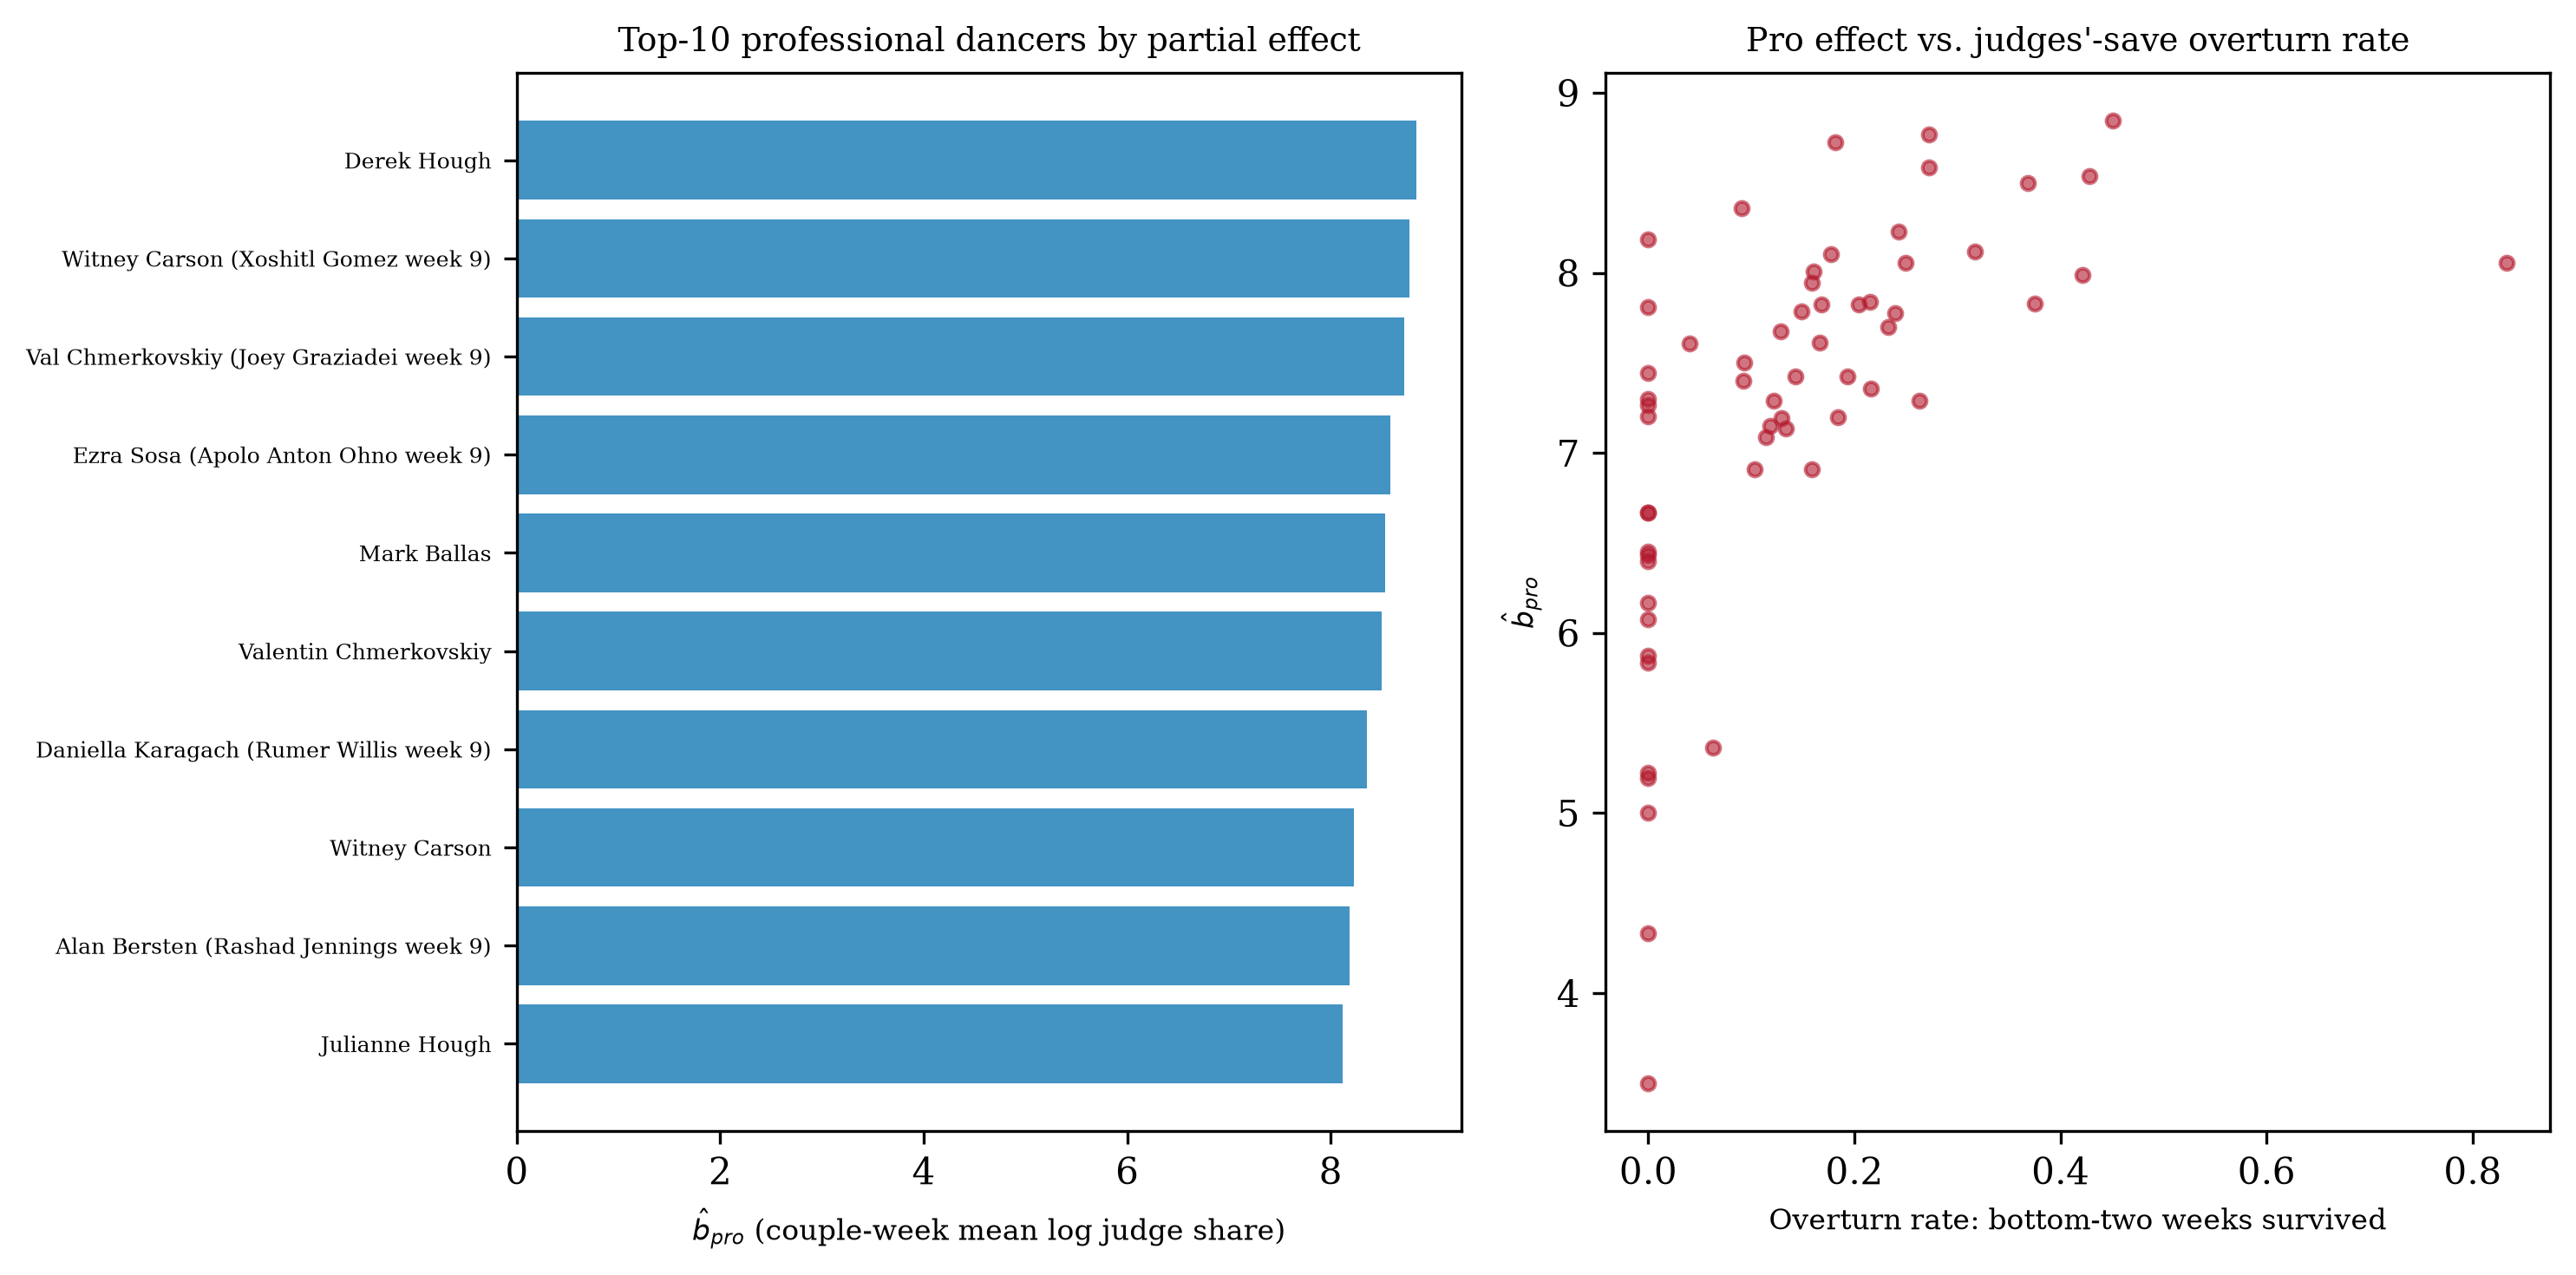
\includegraphics[width=0.85\textwidth]{../02_programming/model_3/figures/fig3_pro_effects.png}
\caption{Professional-dancer effects ($b_{pro}$) with per-dancer couple-week counts and
bottom-two overturn rates. Derek Hough, Mark Ballas, and Val Chmerkovskiy anchor the top
of the distribution; intervals widen for dancers with fewer couple-weeks --- a direct
consequence of mixed-effects shrinkage, not a substantive claim about those dancers.}
\label{fig:pros}
\end{figure}

Figure \ref{fig:pros} makes the pro-dancer hierarchy visible and also displays the
sample-size dimension: dancers with fewer couple-weeks are shrunk toward the mean
because the mixed-effect specification pools them, which is precisely why short-tenure
pros like Charlotte Jorgensen (6 weeks) should be read with caution.

\subsubsection{Leave-one-pro-out stability}

The \texttt{lopo\_refits.csv} table refits the judge channel five times, each excluding
one of the top five pros (Table \ref{tab:lopo}). Excluding Derek Hough moves the refit
intercept from $2.451$ to $2.472$ (a shift of just $0.02$) and leaves the age effect
nearly unchanged ($-0.0012$ vs.\ $-0.0015$ in the full fit). Excluding Mark Ballas
moves the intercept to $2.481$. All five refits agree that the pro-effect ranking is
not an artifact of any single dominant dancer.

\begin{table}[H]
\centering
\caption{Leave-one-pro-out refits of the judge channel (top five pros excluded one at a
time). Stability of the intercept and age effect confirms that the estimated pro
effects are not driven by a single influential dancer.}
\label{tab:lopo}
\small
\begin{tabular}{lrrr}
\toprule
Pro excluded & $b_{pro}$ (of excluded) & Refit intercept & Refit age coef.\\
\midrule
Derek Hough & $8.844$ & $2.472$ & $-0.00120$\\
Witney Carson (wk-9 partner) & $8.770$ & $2.453$ & $-0.00156$\\
Val Chmerkovskiy (wk-9 partner) & $8.723$ & $2.449$ & $-0.00144$\\
Ezra Sosa (wk-9 partner) & $8.588$ & $2.443$ & $-0.00131$\\
Mark Ballas & $8.539$ & $2.481$ & $-0.00209$\\
\bottomrule
\end{tabular}
\end{table}

\subsubsection{Archetype counterfactuals}

\texttt{archetype\_counterfactuals.csv} translates the coefficient vectors into three
concrete casting archetypes (Table \ref{tab:archetypes}): a \emph{young athlete with a
weak pro} ($b_{pro}$ at $-1$ sd; age 24) has predicted $\log(\texttt{Jshare}) = 2.334$
and a survival hazard multiplier of \textbf{0.675} (i.e.\ $\approx$32\% \emph{lower}
weekly elimination hazard than the average cast member), while a \emph{veteran actor
with a star pro} ($b_{pro}$ at $+1$ sd; age 58) has the highest predicted judge channel
($\log \texttt{Jshare} = 2.446$, relative judge share 1.058) but a hazard multiplier of
\textbf{1.460} ($\approx$46\% \emph{higher} weekly elimination hazard). In plain terms:
\textbf{a young athlete with a weak pro buys fan-driven longevity, while a veteran
actor with a star pro buys judge-driven technical marks but not survival.} The average
cast member (age 42, $b_{pro}$ at 0 sd) has a hazard multiplier of 1.015, the
reference level.

\begin{table}[H]
\centering
\caption{Archetype counterfactuals: predicted judge channel and weekly survival hazard
multiplier relative to an average cast member (multiplier $= 1$).}
\label{tab:archetypes}
\small
\begin{tabular}{lrrrrr}
\toprule
Archetype & Age & $b_{pro}$ (sd) & $\log(\texttt{Jshare})$ & rel.\ Jshare & hazard mult.\\
\midrule
Young athlete, weak pro & 24 & $-1$ & $2.334$ & $0.946$ & $\mathbf{0.675}$\\
Average cast member & 42 & $0$ & $2.389$ & $0.999$ & $1.015$\\
Veteran actor, star pro & 58 & $+1$ & $2.446$ & $1.058$ & $\mathbf{1.460}$\\
\bottomrule
\end{tabular}
\end{table}

\subsubsection{Validation}

Four checks: (i) \emph{bootstrap CIs} (\texttt{boot\_ci\_judge\_channel.csv}) exclude
zero for every FDR-significant judge-channel coefficient; (ii) the
\emph{leave-one-pro-out} refits (\texttt{lopo\_refits.csv}) show the pro-effect ranking
is stable to exclusion of each of the top five professionals; (iii) divergence signs
($E_g$ for prior fame, athlete, comedian, social media) are stable across draws and
consistent with the bootstrap; (iv) the planned sensitivity refit excluding
\texttt{fshare\_sd} top-decile rows (master-plan check 4c) was \textbf{not executed},
so divergence estimates are reported without that robustness confirmation and we flag
it as an open robustness item.
